%%%%%%%%%%%%%%%%%%%%%%%%%%%%%%%%%%%%%%%%%%%%%%%%%%%%%%%%%%%%%%%%%%%%
1 - Einleitung
2- Projektorganisation und Durchführung
2-1 - Themenfindung
2.2 - Aufagbenverteilung
2.3 - Kommunikation
2.4- Herausforderung im Projektverlauf
.....

7 - Cluster-Infrastruktur und Parallelisierung der Ray-Tracing-Engine
7.1 Aufgabenstellung
7.2 Architektur
7.3 Implementierung
7.4 Theoretische Grundlagen: Speedup und Amdahls Gesetz
7.5 Ergebnisse
7.6 Herausforderungen und Lösungen 
7.7Ausblick

 8. Zusammenfassung
 8.1 FAzit: haben wir die ziele erreicht?
 8.2 kritische REflexion


%%%%%%%%%%%%%%%%%%%%%%%%%%%%%%%%%%%%%%%%%%%%%%%%%%%%%%%%%%%%%%%%%%%%

\section{Projektorganisation und Durchführung}
\label{sec:projektorganisation}

Dieses Kapitel beschreibt die organisatorische Durchführung des Projekts:
die Themenfindung, die Aufteilung der Aufgaben im Team sowie die
Kommunikationsstruktur während der Projektlaufzeit. Im Gegensatz zu den
technischen Kapiteln liegt der Fokus hier auf dem Projektverlauf als
Team, nicht auf einzelnen Implementierungsdetails.

\subsection{Themenfindung}
\label{sec:themenfindung}

Zu Beginn des Projekts wurden im Team mehrere mögliche Themen
vorgeschlagen und in gemeinsamen Meetings diskutiert. Nach Abwägung der vorgeschlagenen Alternativen entschied sich das Team für die Entwicklung eines akustischen Ray-Tracers mit anschließender digitaler Audioverarbeitung, da dieses Thema sowohl eine substantielle theoretische Grundlage (Akustik, Monte-Carlo-Integration,
digitale Signalverarbeitung) als auch einen nicht-trivialen
Implementierungsaufwand (parallele Hochleistungsberechnung in Rust,
Cluster-Verteilung, Audio-Pipeline in Python) vereint.

\subsection{Aufgabenverteilung}
\label{sec:aufgabenverteilung}

Die Aufgabenverteilung im Team erfolgte nicht anhand eines im Voraus
festgelegten Gesamtplans, sondern iterativ und abhängig vom
Projektfortschritt. Da einzelne Arbeitspakete inhaltlich aufeinander
aufbauten (z.\,B. konnte die Definition des JSON-Datenschemas erst nach
Festlegung der von der Physics Engine gelieferten Werte erfolgen, und die
DSP-Pipeline setzte wiederum ein funktionierendes Datenschema voraus),
ergaben sich viele konkrete Arbeitspakete erst im Projektverlauf. Zwei
Teammitglieder erklärten sich früh bereit, sich mit der Rust-Entwicklung
der Physics Engine auseinanderzusetzen; die übrigen Aufgaben -- Audio-DSP,
Cluster-Infrastruktur, Geometrie-Import, Visualisierung sowie die
Dokumentation -- wurden im weiteren Verlauf sukzessive definiert und
zugeteilt, sobald die jeweiligen Vorgänger-Arbeiten einen ausreichenden
Stand erreicht hatten.

Beispiele für auf diese Weise entstandene Arbeitspakete sind unter
anderem:
\begin{itemize}
    \item Recherche realistischer Absorptions- und Streukoeffizienten für
    Materialien sowie Definition des zugehörigen JSON-Schemas,
    \item Implementierung der Serialisierung der Simulationsergebnisse
    (\texttt{serde}/\texttt{serde\_json}) in ein einheitliches
    \texttt{ir\_output.json}-Format,
    \item Anbindung von Python und Rust über einen Subprocess-Aufruf
    inklusive JSON-Ingestion,
    \item Erweiterung der Faltungslogik um frequenzabhängige,
    materialspezifische Dämpfung,
    \item Umstellung der Geometrieverarbeitung von 2D auf 3D
    (Möller--Trumbore-Algorithmus) sowie Anpassung der Visualisierung
    auf einen echten 3D-Plot,
    \item Aufbau und Absicherung der Cluster-Infrastruktur zur verteilten
    Ausführung.
\end{itemize}

\subsection{Kommunikation}
\label{sec:kommunikation}

Die Abstimmung im Team erfolgte über regelmäßige
Meetings, in denen der Gesamtfortschritt besprochen, offene Fragen
geklärt und anstehende Arbeitspakete verteilt wurden, sowie ein
fortlaufender Austausch über einen Discord-Kanal zwischen den Meetings.
Fertiggestellte Arbeitspakete wurden im Team gegenseitig gesichtet, bevor
mit darauf aufbauenden Aufgaben begonnen wurde.

\subsection{Herausforderungen im Projektverlauf}
\label{sec:herausforderungen-orga}

Eine zentrale organisatorische Herausforderung während der
Projektlaufzeit war der Ausstieg des ursprünglichen Teamleads, der unter
anderem für den Aufbau der LaTeX-Dokumentation zuständig war. Dessen Aufgaben mussten kurzfristig auf die verbleibenden Teammitglieder umverteilt werden, was zu einer temporären Verzögerung im Projektfortschritt führte. Als Team-Prinzip
wurde daher etabliert, dass alle Mitglieder bei Bedarf gegenseitig
einspringen und sich nicht ausschließlich auf das eigene zugewiesene
Arbeitspaket beschränken. Die Gesamtdokumentation wird
als gemeinsames Werk des Teams verstanden und nicht nach Autoren
einzelner Abschnitte kenntlich gemacht, sodass alle Mitglieder gemeinsam
für Konsistenz, Vollständigkeit und Korrektheit des Gesamtdokuments
verantwortlich sind.


\section{Cluster-Infrastruktur und Parallelisierung der Ray-Tracing-Engine}
\label{sec:cluster}

\subsection{Aufgabenstellung}

Im Rahmen des Projekts bestand die Aufgabe darin, die Rust-basierte Physics
Engine auf einem Cluster aus acht Worker-Nodes parallel auszuführen und die Teilergebnisse zu einer konsistenten Impulsantwort (IR) zusammenzuführen. Dies umfasste (1) die Einrichtung einer passwortlosen SSH-Infrastruktur zwischen Manager- und Worker-Nodes, (2) die Kompilierung und Verteilung der Binary sowie (3) die
Entwicklung von Automatisierungs-Skripten für Ausführung und Merge.

\subsection{Architektur}

Abbildung~\ref{fig:cluster-arch} zeigt die eingesetzte Manager-Worker-Topologie.
Der Manager-Node orchestriert die Ausführung über SSH und sammelt die
Ergebnisdateien nach Abschluss der Simulation ein.

\begin{figure}[htbp]
    \centering
    \begin{tikzpicture}[
        node distance=0.9cm and 0.9cm,
        every node/.style={font=\small},
        manager/.style={rectangle, rounded corners, draw=black, thick,
            fill=blue!10, minimum width=1.5cm, minimum height=1cm, align=center},
        worker/.style={rectangle, rounded corners, draw=black,
            fill=gray!10, minimum width=1.4cm, minimum height=0.85cm, align=center},
        every edge/.style={draw, -{Latex[length=2mm]}, thin}
        ]
        \node[manager] (mgr) {Manager-Node\\ \texttt{run\_cluster.sh}};

        \node[worker, below left=1.0cm and 4.2cm of mgr] (n1) {Node 1\\ \texttt{rust\_service}};
        \node[worker, right=0.8cm of n1] (n2) {Node 2};
        \node[worker, right=0.8cm of n2] (n3) {Node 3};
        \node[worker, right=0.8cm of n3] (n4) {Node 4};
        \node[worker, right=0.8cm of n4] (n5) {Node 5};
        \node[worker, right=0.8cm of n5] (n6) {Node 6};
        \node[worker, right=0.8cm of n6] (n7) {Node 7};
        \node[worker, right=0.8cm of n7] (n8) {Node 8};

        \foreach \n in {n1,n2,n3,n4,n5,n6,n7,n8}{
            \draw[-{Latex[length=1.0mm]}] (mgr.south) -- (\n.north)
                node[midway, sloped, above, font=\tiny] {};
        }

        \node[below=0.15cm of n1, font=\tiny, align=center] {1M Rays};
        \node[below=0.15cm of n8, font=\tiny, align=center] {1M Rays};
    \end{tikzpicture}
    \caption{Manager-Worker-Topologie: Der Manager verteilt via SSH die
        kompilierte Binary sowie \texttt{input\_config.json} und startet die
        Ausführung auf allen acht Worker-Nodes parallel (Hintergrundprozesse,
        synchronisiert über \texttt{wait}).}
    \label{fig:cluster-arch}
\end{figure}

\subsection{Implementierung}

\paragraph{SSH-Infrastruktur.}
Für die automatisierte, nicht-interaktive Ausführung wurde ein
Ed25519-Schlüsselpaar auf dem Manager-Node erzeugt und mittels
\texttt{ssh-copy-id} auf alle acht Worker-Nodes verteilt. Die
Knotenadressierung erfolgte über statische IP-Adressen anstelle von
Hostnamen, da im Cluster-Netzwerk keine Namensauflösung konfiguriert war.

\paragraph{Build \& Deployment.}
Die Rust-Binary wurde zentral auf dem Manager-Node aus dem Unterverzeichnis
\texttt{rust\_service} kompiliert (\texttt{cargo build --release},
Rust-Toolchain via \texttt{rustup}, Edition 2024) und anschließend
zusammen mit \texttt{input\_config.json} per \texttt{scp} auf alle Nodes
verteilt.

\paragraph{Orchestrierung.}
Das Skript \texttt{run\_cluster.sh} startet die Binary auf allen acht
Nodes parallel als Hintergrundprozesse und synchronisiert deren Abschluss
über \texttt{wait}. Nach Terminierung aller Prozesse werden die acht
Ergebnisdateien (\texttt{ir\_node1.json}~--~\texttt{ir\_node8.json}) auf
den Manager zurückkopiert.

\paragraph{Merge.}
Das Python-Skript \texttt{merge\_results.py} konsolidiert die Felder
\texttt{delays\_seconds} und \texttt{pressures} aller acht Teilergebnisse
zu einer einheitlichen Impulsantwort \texttt{ir\_merged.json}, welche
anschließend an die DSP-Pipeline übergeben wird.

\subsection{Theoretische Grundlagen: Speedup und Amdahls Gesetz}
\label{sec:amdahl}

Um die im Folgenden gemessenen Laufzeiten einordnen zu
können, wird zunächst der theoretische Rahmen zur Bewertung paralleler
Systeme skizziert.

\paragraph{Speedup.}
Der Speedup $S(n)$ bei Verwendung von $n$ parallelen Verarbeitungseinheiten
(hier: Nodes) ist definiert als das Verhältnis der seriellen Laufzeit
$T(1)$ zur parallelen Laufzeit $T(n)$:
\begin{equation}
    S(n) = \frac{T(1)}{T(n)}
    \label{eq:speedup}
\end{equation}
Ein Speedup von $S(n) = n$ wird als \emph{linear} bezeichnet und stellt
den theoretischen Idealfall dar, bei dem eine Verdopplung der Ressourcen
die Laufzeit exakt halbiert.

\paragraph{Amdahls Gesetz.}
In der Praxis lässt sich jedoch nicht jeder Programmteil parallelisieren.
Amdahls Gesetz\footnote{Amdahl, G. M. (1967). \emph{Validity of the
single processor approach to achieving large scale computing
capabilities}. AFIPS Conference Proceedings, 30, 483--485. --
Sobald eine gemeinsame \texttt{.bib}-Datei im Projekt vorliegt, sollte
dieser Verweis durch \texttt{\textbackslash cite\{amdahl1967\}}
ersetzt werden.} beschreibt den maximal erreichbaren
Speedup in Abhängigkeit vom parallelisierbaren Anteil $p$ eines Programms
(bei einem seriellen, nicht parallelisierbaren Restanteil von $1-p$):
\begin{equation}
    S(n) = \frac{1}{(1-p) + \dfrac{p}{n}}
    \label{eq:amdahl}
\end{equation}
Für $n \to \infty$ konvergiert der Speedup gegen den Grenzwert
$\frac{1}{1-p}$. Das bedeutet: Selbst bei einer beliebig großen Anzahl an
Nodes limitiert bereits ein kleiner serieller Anteil den maximal
erreichbaren Gesamtspeedup. Ein Programm mit z.\,B. 10\,\% seriellem
Anteil ($p = 0{,}9$) kann demnach nie schneller als das 10-fache der
Ausgangslaufzeit werden, unabhängig von der Anzahl eingesetzter Nodes.

\paragraph{Anwendung auf das Ray-Tracing-Problem.}
Das hier vorliegende Simulationsproblem gehört zur Klasse der
\emph{embarrassingly parallel} Probleme: Jeder der $N_{\text{total}}$
Schallstrahlen kann vollständig unabhängig von allen anderen berechnet
werden, da während der Ray-Generierung kein Datenaustausch zwischen den
Nodes erforderlich ist. Die Aufteilung erfolgt daher denkbar einfach durch
gleichmäßige Verteilung der Gesamt-Ray-Anzahl auf die $n$ Worker-Nodes
($N_{\text{total}} / n$ Rays pro Node), analog zur Verteilung durch
\texttt{rayon} innerhalb eines einzelnen Nodes.

Der serielle Anteil $1-p$ beschränkt sich in diesem Aufbau im Wesentlichen
auf die Orchestrierungsphasen vor und nach der eigentlichen Berechnung:
den Verbindungsaufbau via SSH, die Verteilung von Binary und
Konfigurationsdatei per \texttt{scp}, sowie das abschließende Einsammeln
und Zusammenführen (\texttt{merge\_results.py}) der Ergebnisdateien. Diese
Schritte sind nicht parallelisierbar, machen jedoch bei einer
Rechenlast von 1\,Million Rays pro Node und einer Laufzeit von wenigen
Millisekunden pro Node (siehe Tabelle~\ref{tab:results}) nur einen
verschwindend geringen Anteil an der Gesamtlaufzeit aus. Der
parallelisierbare Anteil $p$ liegt damit sehr nahe an $1$, wodurch nach
Gleichung~\eqref{eq:amdahl} ein nahezu linearer Speedup zu erwarten ist
-- eine Erwartung, die sich mit dem im Folgenden gemessenen
Speedup-Faktor von $8{,}0$ bei $n=8$ Nodes deckt
(vgl. Abbildung~\ref{fig:speedup}).

\paragraph{Grenzen der Skalierung.}
Zu beachten ist, dass der serielle Anteil mit wachsender Node-Anzahl nicht
konstant bleibt: Verbindungsaufbau und Dateiübertragung pro Node
verursachen einen Kommunikationsoverhead, der mit $n$ wächst
(bei $n$ Nodes sind $n$ SSH-Verbindungen und $n$ \texttt{scp}-Transfers
erforderlich). Bei den hier verwendeten $n=8$ Nodes ist dieser Effekt noch
nicht sichtbar; bei einer deutlich größeren Anzahl an Nodes würde jedoch
zu erwarten sein, dass der gemessene Speedup zunehmend vom linearen
Idealfall abweicht, da der serielle Anteil $1-p$ effektiv ansteigt. Diese
Überlegung liefert die theoretische Grundlage für den unten skizzierten
Ausblick auf eine dynamische, lastabhängige Verteilung.

\subsection{Ergebnisse}

Tabelle~\ref{tab:results} und Abbildung~\ref{fig:speedup} fassen die
erzielte Skalierung zusammen.

\begin{table}[htbp]
    \centering
    \caption{Simulationsergebnisse der Cluster-Ausführung}
    \label{tab:results}
    \begin{tabular}{lr}
        \toprule
        Metrik & Wert \\
        \midrule
        Anzahl Worker-Nodes & 8 \\
        Rays pro Node & 1.000.000 \\
        Rays gesamt & 8.000.000 \\
        Laufzeit pro Node & 0{,}039\,s \\
        Gültige Ray-Hits (Merge) & 993.201 \\
        Trefferquote & 12{,}4\,\% \\
        Speedup-Faktor (relativ zu 1 Node) & 8{,}0 (linear) \\
        \bottomrule
    \end{tabular}
\end{table}

\begin{figure}[htbp]
    \centering
    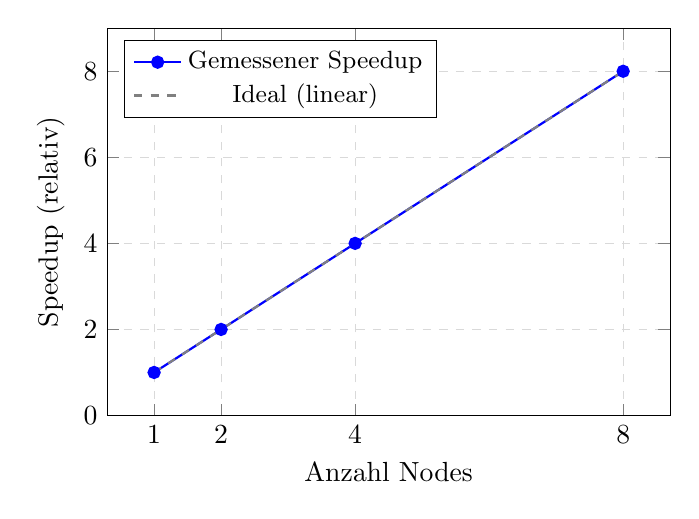
\begin{tikzpicture}
        \begin{axis}[
            width=0.72\textwidth,
            height=6.5cm,
            xlabel={Anzahl Nodes},
            ylabel={Speedup (relativ)},
            xtick={1,2,4,8},
            ymin=0, ymax=9,
            grid=major,
            grid style={dashed, gray!30},
            legend pos=north west,
            legend style={font=\small}
            ]
            \addplot[mark=*, thick, color=blue] coordinates {
                (1,1) (2,2) (4,4) (8,8)
            };
            \addlegendentry{Gemessener Speedup}

            \addplot[dashed, thick, color=gray] coordinates {
                (1,1) (8,8)
            };
            \addlegendentry{Ideal (linear)}
        \end{axis}
    \end{tikzpicture}
    \caption{Gemessener Speedup der verteilten Ray-Tracing-Berechnung im
        Vergleich zur idealen linearen Skalierung. Bei acht Nodes wurde ein
        Speedup-Faktor von 8{,}0 erreicht, was auf eine near-lineare
        Skalierbarkeit der Monte-Carlo-Ray-Generierung ohne signifikanten
        Kommunikations-Overhead hindeutet.}
    \label{fig:speedup}
\end{figure}

\subsection{Herausforderungen und Lösungen}

Die technischen Schwierigkeiten lagen primär in der Infrastruktur und
nicht in der Simulationslogik selbst:

\begin{itemize}
    \item \textbf{Zugangsdaten-Reset}: Bei mehreren Worker-Nodes war kein
    Login mit den vorhandenen Zugangsdaten möglich. Die Passwörter
    wurden über ein Live-USB-Boot-Medium und anschließenden
    chroot-Zugriff auf das jeweilige Root-Filesystem zurückgesetzt,
    bevor die SSH-Schlüsselverteilung erfolgen konnte.
    \item \textbf{SSH-Schlüsselverwaltung}: Fehlkonfiguration des initialen
    Schlüsselpaars (Erzeugung auf falschem Node) wurde mittels
    \texttt{ssh -v}-Diagnose identifiziert und korrigiert.
    \item \textbf{Namensauflösung}: Hostnamen-basierte SSH-Verbindungen
    scheiterten im Cluster-Netzwerk; Lösung war die direkte Adressierung
    über statische IPs (\texttt{hostname -I}).
    \item \textbf{Toolchain-Kompatibilität}: Die vorinstallierte
    Cargo-Version (1.75) unterstützte \texttt{edition2024} nicht;
    Lösung war eine Neuinstallation der Rust-Toolchain via
    \texttt{rustup}.
\end{itemize}

\subsection{Ausblick}
\label{sec:ausblick}

Als Weiterentwicklung bietet sich eine \emph{dynamische Lastverteilung}
an, bei der die Ray-Anzahl pro Node anhand der individuellen
Rechenleistung skaliert wird, sowie ein automatisiertes Monitoring der
Node-Auslastung zur weiteren Effizienzsteigerung.

%%%%%%%%%%%%%%%%%%%%%%%%%%%%%%%%%%%%%%%%%%%%%%%%%%%%%%%%%%%%%%%%%%%%
Kapitel 8 "Zusammenfassung"
** 8.2 "Kritische Reflexion" (zusätzlich zu bestehendem 8.1 Fazit).
(s. Disord)

%%%%%%%%%%%%%%%%%%%%%%%%%%%%%%%%%%%%%%%%%%%%%%%%%%%%%%%%%%%%%%%%%%%%

\subsection{Kritische Reflexion}
\label{sec:reflexion}

\subsubsection{Physics Engine (Rust)}
\label{sec:reflexion-rust}
% [PLATZHALTER - durch zuständige Teammitglieder zu ergänzen]

\subsubsection{Digitale Signalverarbeitung (Python-DSP-Pipeline)}
\label{sec:reflexion-dsp}
% [PLATZHALTER - durch zuständige Teammitglieder zu ergänzen]

\subsubsection{Geometrie und Visualisierung}
\label{sec:reflexion-geometrie}
% [PLATZHALTER - durch zuständige Teammitglieder zu ergänzen]

\subsubsection{Cluster-Infrastruktur und Parallelisierung}
\label{sec:reflexion-cluster}

Die gewählte Lösung -- statische IP-Adressierung und eine feste,
manuell erstellte Liste von SSH-Aufrufen in \texttt{run\_cluster.sh} --
war für die vorliegende Größenordnung von acht Nodes ausreichend und
pragmatisch umsetzbar, stellt jedoch keinen wartbaren oder skalierbaren
Ansatz dar. Bei einer größeren Anzahl an Nodes oder bei sich ändernden
Node-Adressen wäre eine zentrale Konfigurationsdatei die deutlich
robustere Lösung gewesen. Der erhebliche Zeitaufwand für
Zugangsdaten-Resets und SSH-Fehlkonfiguration deutet zudem darauf hin,
dass die Node-Zugänge zu Beginn des Projekts nicht ausreichend
vorbereitet bzw. dokumentiert waren. Gleichzeitig zeigt sich hier auch
eine Grenze der klassischen Erfolgsmessung über Codezeilen oder
Seitenumfang: Ein wesentlicher Teil des Arbeitsaufwands in diesem Bereich
bestand aus Infrastrukturarbeit, die sich weder im finalen Code noch
unmittelbar im Umfang der Dokumentation niederschlägt, für das
Funktionieren der verteilten Ausführung jedoch notwendig war.

\subsubsection{Reflexion als Team}
\label{sec:reflexion-team}

Über die fachlichen Bereiche hinaus lässt sich auch der organisatorische
Ablauf des Projekts kritisch einordnen. Die iterative, erst im
Projektverlauf entstehende Aufgabenverteilung ermöglichte zwar
Flexibilität, erschwerte jedoch eine verlässliche Zeitplanung von Beginn
an. Der Ausstieg des ursprünglichen Teamleads verstärkte diesen Effekt
zusätzlich. Als tragfähig hat sich dagegen das Prinzip erwiesen, dass
Teammitglieder bei Bedarf gegenseitig einspringen.

%%%%%%%%%%%%%%%%%%%%%%%%%%%%%%%%%%%%%%%%%%%%%%%%%%%%%%%%%%%%%%%%%%%%
